\chapter*{Anexo B: Resultados completos del banco de pruebas}
\addcontentsline{toc}{chapter}{Anexo B: Resultados completos del banco de pruebas}
\label{cap:anexo_benchmark}

\setcounter{section}{0}
\renewcommand{\thesection}{B.\arabic{section}}

Este anexo reúne los resultados medidos de la campaña descrita en el
Capítulo~\ref{cap:visualizacion}, de los que el cuerpo del documento solo
cita las cifras necesarias para su argumento. Todas las cifras proceden de
los registros de ejecución de la campaña, procesados por el módulo de
informes del repositorio, y la versión completa, con todas las columnas
medidas, está en \path{docs/benchmark/results.md}.

\section{Volumen de datos por escala}
\label{sec:anexo_benchmark_datos}

Cada escala contiene a la anterior, de modo que los registros de ORCID y los
currículos sintéticos de la escala menor forman parte de la mayor. La
Tabla~\ref{tab:anexo_benchmark_escalas} recoge lo que se aterrizó realmente
en cada una. La tasa de rechazo se mantiene alrededor del 2,7\% en las tres
escalas, lo que indica que la composición de los datos no cambia con el
volumen.

\begin{table}[H]
  \centering
  \footnotesize
  \renewcommand{\arraystretch}{1.1}
  \begin{tabular}{
    p{0.07\textwidth}
    >{\raggedright\arraybackslash}p{0.22\textwidth}
    >{\raggedright\arraybackslash}p{0.17\textwidth}
    p{0.08\textwidth}
    >{\raggedright\arraybackslash}p{0.14\textwidth}
    p{0.12\textwidth}}
    \hline
    \textbf{Escala} & \textbf{Registros masivos de ORCID, con rechazo} & \textbf{CVN sintéticos, con identificador} & \textbf{API} & \textbf{Registros de persona} & \textbf{Tamaño} \\
    \hline
    1x & 19\,469, 2,66\% & 11\,000, 7\,800 & 200 & 30\,669 & 2,82 GB \\
    2x & 38\,920, 2,70\% & 22\,000, 15\,500 & 200 & 61\,120 & 5,49 GB \\
    4x & 77\,868, 2,67\% & 44\,000, 31\,003 & 200 & 122\,068 & 10,94 GB \\
    \hline
  \end{tabular}
  \caption{Datos aterrizados en cada escala del banco de pruebas.}
  \label{tab:anexo_benchmark_escalas}
\end{table}

\section{Tiempos, aceleración y eficiencia por trabajo}
\label{sec:anexo_benchmark_tiempos}

Las tres tablas siguientes dan, para cada combinación de escala y número de
ejecutores, el número de ejecuciones válidas, la mediana y el rango de
tiempo de aplicación, la aceleración respecto a un ejecutor, su eficiencia
y el uso medio de procesador del sistema. Una celda vacía indica que esa
configuración no produjo ninguna ejecución válida.

\begin{table}[H]
  \centering
  \footnotesize
  \setlength{\tabcolsep}{4pt}
  \renewcommand{\arraystretch}{1.05}
  \begin{tabular}{p{0.07\textwidth} p{0.08\textwidth} p{0.09\textwidth} p{0.1\textwidth} p{0.17\textwidth} p{0.11\textwidth} p{0.1\textwidth} p{0.08\textwidth}}
    \hline
    \textbf{Escala} & \textbf{Ejec.} & \textbf{Válidas} & \textbf{Mediana, s} & \textbf{Rango, s} & \textbf{Acel.} & \textbf{Efic.} & \textbf{CPU, \%} \\
    \hline
    1x & 1 & 1 & 337,1 & 337,1 & 1,00 & 1,00 & 11,4 \\
    1x & 2 & 3 & 224,4 & 215,5 a 235,5 & 1,50 & 0,75 & 18,2 \\
    1x & 4 & 3 & 206,8 & 204,3 a 421,0 & 1,63 & 0,41 & 28,1 \\
    2x & 1 & 0 & -- & -- & -- & -- & -- \\
    2x & 2 & 1 & 383,0 & 383,0 & -- & -- & 18,0 \\
    2x & 4 & 2 & 742,1 & 405,3 a 1\,078,9 & -- & -- & 23,0 \\
    4x & 1 & 0 & -- & -- & -- & -- & -- \\
    4x & 2 & 0 & -- & -- & -- & -- & -- \\
    4x & 4 & 1 & 1\,125,1 & 1\,125,1 & -- & -- & 19,8 \\
    \hline
  \end{tabular}
  \caption{Validación y normalización de bronze a silver.}
  \label{tab:anexo_benchmark_silver}
\end{table}

\begin{table}[H]
  \centering
  \footnotesize
  \setlength{\tabcolsep}{4pt}
  \renewcommand{\arraystretch}{1.05}
  \begin{tabular}{p{0.07\textwidth} p{0.08\textwidth} p{0.09\textwidth} p{0.1\textwidth} p{0.17\textwidth} p{0.11\textwidth} p{0.1\textwidth} p{0.08\textwidth}}
    \hline
    \textbf{Escala} & \textbf{Ejec.} & \textbf{Válidas} & \textbf{Mediana, s} & \textbf{Rango, s} & \textbf{Acel.} & \textbf{Efic.} & \textbf{CPU, \%} \\
    \hline
    1x & 1 & 3 & 78,6 & 77,4 a 80,5 & 1,00 & 1,00 & 14,8 \\
    1x & 2 & 3 & 74,5 & 71,4 a 76,4 & 1,06 & 0,53 & 22,7 \\
    1x & 4 & 3 & 85,8 & 85,1 a 89,5 & 0,92 & 0,23 & 32,2 \\
    2x & 1 & 3 & 115,0 & 113,5 a 121,3 & 1,00 & 1,00 & 13,1 \\
    2x & 2 & 3 & 102,5 & 102,4 a 104,3 & 1,12 & 0,56 & 19,0 \\
    2x & 4 & 3 & 109,1 & 107,5 a 109,5 & 1,05 & 0,26 & 29,3 \\
    4x & 1 & 3 & 302,4 & 268,1 a 384,4 & 1,00 & 1,00 & 8,7 \\
    4x & 2 & 2 & 280,2 & 279,5 a 280,9 & 1,08 & 0,54 & 11,2 \\
    4x & 4 & 3 & 257,6 & 196,7 a 259,0 & 1,17 & 0,29 & 18,5 \\
    \hline
  \end{tabular}
  \caption{Cálculo de indicadores de silver a gold.}
  \label{tab:anexo_benchmark_gold}
\end{table}

\begin{table}[H]
  \centering
  \footnotesize
  \setlength{\tabcolsep}{4pt}
  \renewcommand{\arraystretch}{1.05}
  \begin{tabular}{p{0.07\textwidth} p{0.08\textwidth} p{0.09\textwidth} p{0.1\textwidth} p{0.17\textwidth} p{0.11\textwidth} p{0.1\textwidth} p{0.08\textwidth}}
    \hline
    \textbf{Escala} & \textbf{Ejec.} & \textbf{Válidas} & \textbf{Mediana, s} & \textbf{Rango, s} & \textbf{Acel.} & \textbf{Efic.} & \textbf{CPU, \%} \\
    \hline
    1x & 1 & 3 & 69,3 & 62,9 a 72,8 & 1,00 & 1,00 & 8,3 \\
    1x & 2 & 3 & 77,0 & 74,3 a 77,9 & 0,90 & 0,45 & 11,1 \\
    1x & 4 & 3 & 87,2 & 83,8 a 88,9 & 0,79 & 0,20 & 15,6 \\
    2x & 1 & 3 & 121,1 & 116,5 a 137,9 & 1,00 & 1,00 & 8,3 \\
    2x & 2 & 3 & 126,0 & 117,6 a 128,6 & 0,96 & 0,48 & 8,6 \\
    2x & 4 & 3 & 141,9 & 136,6 a 164,3 & 0,85 & 0,21 & 11,2 \\
    4x & 1 & 3 & 61,1 & 60,6 a 61,3 & 1,00 & 1,00 & 11,2 \\
    4x & 2 & 3 & 62,2 & 58,7 a 62,2 & 0,98 & 0,49 & 13,8 \\
    4x & 4 & 3 & 69,8 & 68,4 a 71,2 & 0,88 & 0,22 & 19,2 \\
    \hline
  \end{tabular}
  \caption{Publicación de gold en PostgreSQL.}
  \label{tab:anexo_benchmark_publish}
\end{table}

Tres rasgos de estas tablas importan para interpretarlas. Primero, la
aceleración de silver solo existe a escala base, porque a escalas mayores
las configuraciones de uno y dos ejecutores agotan su memoria y no producen
ejecuciones válidas con las que calcularla. Segundo, el rango de la
configuración de cuatro ejecutores a escala base es muy amplio, con un
máximo de 421,0 segundos frente a una mediana de 206,8, y esa dispersión es
la razón por la que se repitió cada punto tres veces. Tercero, la
publicación a escala cuádruple tarda menos que a escala doble, lo que
confirma que su tiempo depende del número de tablas publicadas y no del
volumen de filas que contienen.

\begin{figure}[H]
  \centering
  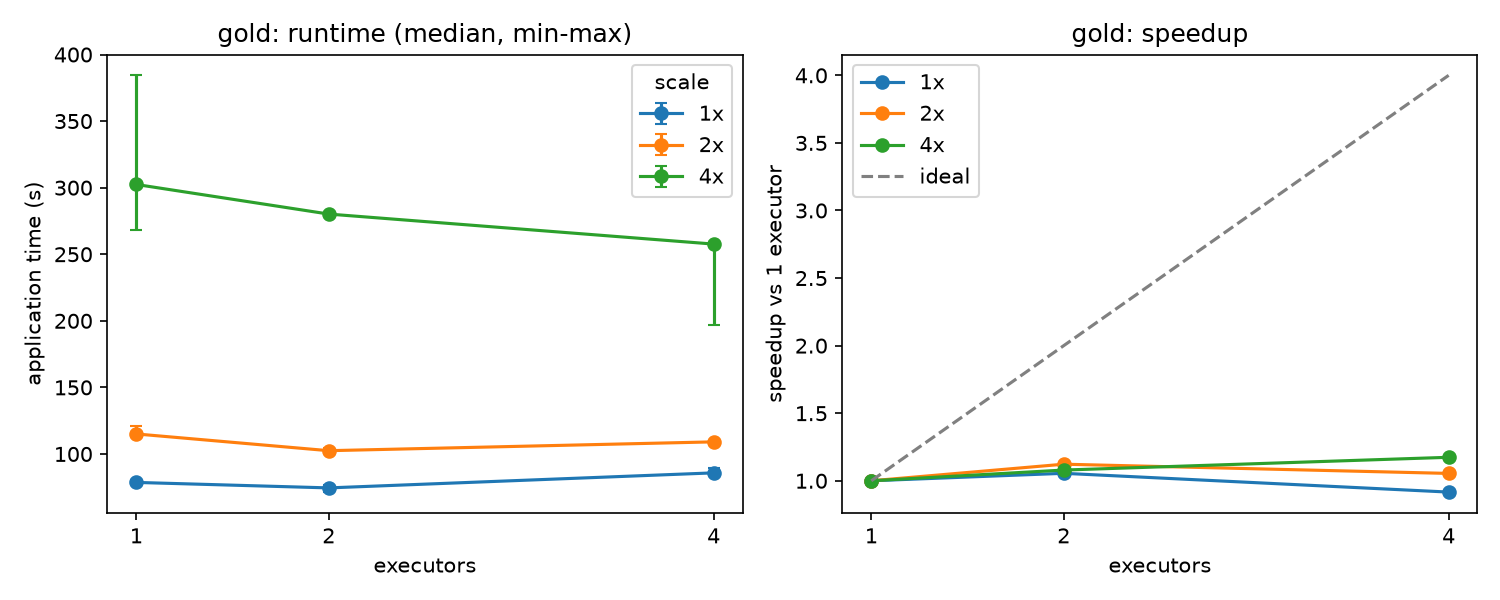
\includegraphics[width=\textwidth]{figs/benchmark_gold.png}
  \caption{Tiempo de ejecución y aceleración del cálculo de indicadores.}
  \label{fig:anexo_benchmark_gold}
\end{figure}

\section{Ejecuciones excluidas}
\label{sec:anexo_benchmark_excluidas}

Una ejecución se excluye de las cifras cuando no es comparable con las
demás. El informe de la campaña lista cada exclusión con su causa, y todas
ellas pertenecen a una de las clases siguientes:

\begin{itemize}
  \item \textbf{Agotamiento de memoria de un ejecutor.} Es el límite
  determinista descrito en el Capítulo~\ref{cap:visualizacion}, que afecta
  a un ejecutor desde el doble de volumen y a dos ejecutores a cuádruple
  volumen. Una vez confirmado en dos intentos sin ningún éxito, la campaña
  deja de repetir esa configuración.
  \item \textbf{Cierre abrupto de un ejecutor en gold.} Ocurrió una sola vez,
  con dos ejecutores a cuádruple volumen, y no es determinista.
  \item \textbf{Registro de eventos ilegible.} Afectó a una ejecución de
  silver con cuatro ejecutores a cuádruple volumen.
  \item \textbf{Ejecutores huérfanos atribuidos a otra ejecución.} Nueve
  ejecuciones de publicación a cuádruple volumen se marcaron como excluidas
  por pods ejecutores que pertenecían a una ejecución anterior fallida. Se
  corrigieron a mano, y cada registro conserva una nota con la prueba de la
  corrección.
\end{itemize}

\section{Corrección del resultado entre configuraciones}
\label{sec:anexo_benchmark_correccion}

Para cada escala y trabajo, las configuraciones que sí produjeron salida
dieron la misma huella de contenido, con independencia del número de
ejecutores. La Tabla~\ref{tab:anexo_benchmark_digest} resume la comprobación.

\begin{table}[H]
  \centering
  \footnotesize
  \renewcommand{\arraystretch}{1.1}
  \begin{tabular}{
    p{0.1\textwidth}
    >{\raggedright\arraybackslash}p{0.2\textwidth}
    >{\raggedright\arraybackslash}p{0.22\textwidth}
    >{\raggedright\arraybackslash}p{0.22\textwidth}}
    \hline
    \textbf{Escala} & \textbf{Salida} & \textbf{Ejecutores sin salida} & \textbf{Huellas idénticas} \\
    \hline
    1x y 2x & Gold y publicación & Ninguno & Sí \\
    1x & Silver & Ninguno & Sí \\
    2x & Silver & 1 ejecutor & Sí entre los restantes \\
    4x & Gold y publicación & Ninguno & Sí \\
    4x & Silver & 1 y 2 ejecutores & No aplicable, solo uno produjo salida \\
    \hline
  \end{tabular}
  \caption{Comprobación de igualdad de contenido entre configuraciones.}
  \label{tab:anexo_benchmark_digest}
\end{table}
